\documentclass[titlepage]{article}
\usepackage[bottom=3cm, right=3cm, left=3cm, top=3cm]{geometry}
\usepackage {graphicx}
\usepackage{caption}
%opening
\title{%
	Practical Machine Learning\\
	
	\vspace*{2em}
	\LARGE Exercise 1 \\
	Spring 2024}
\author{Lisa Stafford}
\date{January 31, 2024}

\begin{document}
	
	\maketitle
	
	\captionsetup{
		format = plain,
		font = footnotesize,
		labelfont = sc
	}
	
	\section*{Abstract}
	Since this is simply a warm up assignment, I am just approaching this assignment with how new or naive users typically start out with respect to machine learning and the most common mistakes that result in very bad and non-performant models.  Since a lot of this is initially exploratory a simple ML model was created using data obtained from the UCI Machine Learning Repository, and consists of a wine quality dataset \cite{dataset1}.  At this stage in the class, minimal data processing is performed.  A simple regression model is built to predict wine quality from the sklearn linear regression model library, then we perform rounding on the predictions, and follow that up with a logistic regression model, and then a support vector machine classification model using a linear kernel.  Each model is built partitioning data with 75\% of data for training and 25\% for testing.  Afterwards, performance is compared between models by comparing a few evaluation metrics. 
	
	\section*{Linear Regression Model}
	This initial exercise uses the most basic of models (A Linear Regression Model). It is recognized that this is far from an ideal model for this particular prediction problem and data set. The idea was to show a very naively developed model, which should result in poor performance, and then explore very basic ways in which we can improve upon it.	Initially we are not even setting this up as a classification model - we're just performing linear regression on what is essentially a classification problem. Which many naive to machine learning actually do quite frequently.
	
	\subsection*{Evaluation Metrics}
	We use the following out of the box metrics from scikitlearn \cite{scikitlearn}:
	\begin{enumerate}
		\item  Model Prediction Score: Per SciKitLearn's Website \cite{scikitlearn}, The accuracy() method "returns the mean accuracy on the given data and labels." Additionally, when performing multi label classification, "this references the subset accuracy which is a harsh metric since it requires each that each label set be correctly predicted for each sample". This particular score is used in this situation to determine the accuracy of prediction on the training data.
	
		\item Explained Variance Score: Per SciKitLearn's Website \cite{scikitlearn}, This metric essentially represents the amount of variation in the original dataset that our model is able to explain.
		
		\item MSE Score: Per SciKitLearn's Website \cite{scikitlearn}, this calculates the mean squared error regression loss on the model.
		
		\item R2 Score: Per SciKitLearn's Website \cite{scikitlearn}, this returns the coefficient of determination on the regression model.
	\end{enumerate}
	
	\subsection*{Accuracy}
	The above scores are all metrics to compute the accuracy of the overall model. Run output is as follows:\\
	\begin{center}
		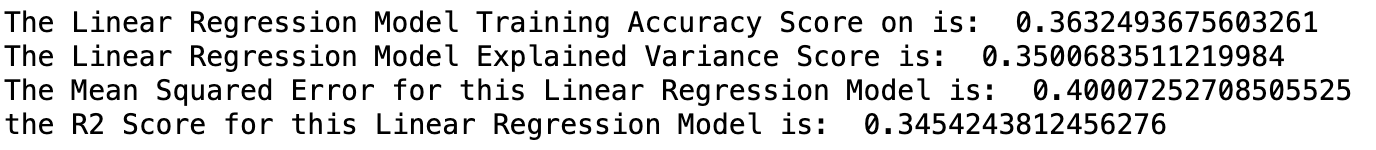
\includegraphics[width=.75\textwidth]{img/img1.png}\newline
		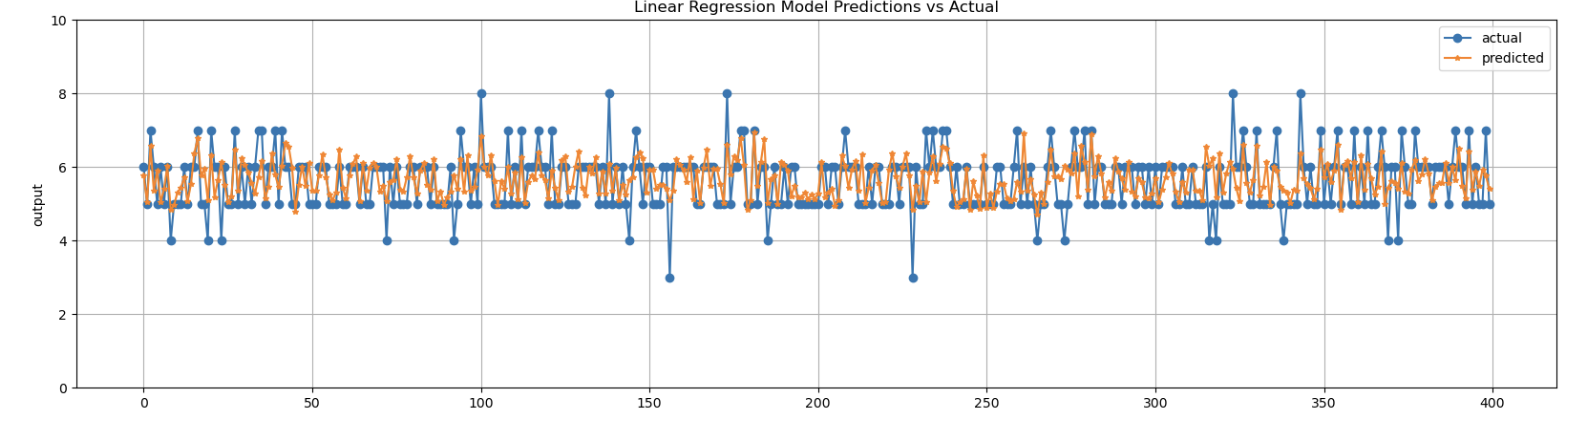
\includegraphics[width=.75\textwidth]{img/img2.png}
	\end{center}
	Additionally, the linear regression model in general is very bad at predicting lower quality wines. All predicted values tend to fall between 5 and 7, and no values under quality 5 are ever predicted correctly.  Even if you round values to the nearest whole number, the predicted values only predict two classes, resulting in a similarly bad classification model and failing to predict any outliers as shown for the following two graphics: 
	\begin{center}
		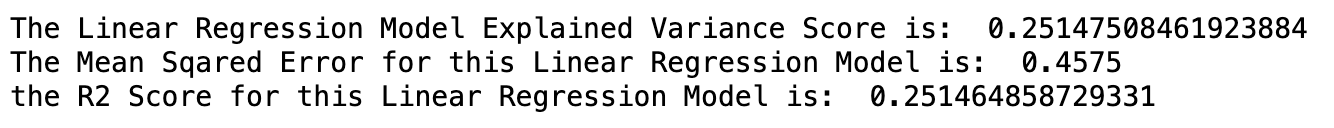
\includegraphics[width=.75\textwidth]{img/img3.png}\newline
		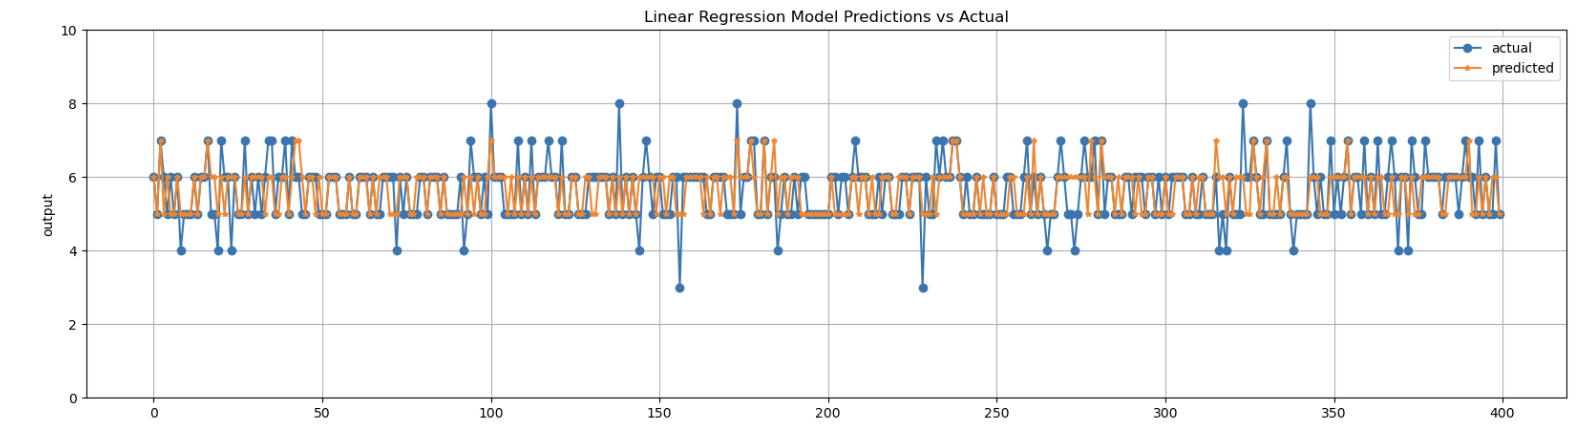
\includegraphics[width=.75\textwidth]{img/img4.png}
	\end{center}
		\subsection*{Summary}
		The simple Linear Regression model is a classical model providing a line for ordinary least squares linear regression on the dataset. The model as developed is not a good predictor of wine quality and fails to accurately predict true wine quality in a majority of cases on test data.  Additionally, it was never meant to predict classifications.  It simply outputs a continuous value, which does not meet the requirements of prediction problem.

\section*{Logistic Regression Model}
This regression exercise uses a logistic regression model detailed on scikit-learn.  This does a much better job of predicting values than the prior Linear Model. Additionally, the logistic regression model uses the $model\_selection.GridSearchCV()$ Optimizer  "to implement a fit and score method and apply them optimized by cross validated grid-search over the parameter grid" that is specified. Ideally, this should come up with the best set of hyperparameters from those listed in the parameter grid to optimize the model for Logistic Regression. The specific hyperparameters are selected because they support classification of multi-class datasets.

	\subsection*{Evaluation Metrics Used}
	For the Logistic Regression Model, we use evaluate with the following:  
	\begin{enumerate}
		\item Model Prediction Score: Per SciKitLearn's Website\cite{scikitlearn}, The accuracy() method "returns the mean accuracy on the given data and labels." Additionally, when performing multi label classification, "this references the subset accuracy which is a harsh metric since it requires each that each label set be correctly predicted for each sample".
		\item Accuracy Score: Per SciKitLearn's Website\cite{scikitlearn}, This metric represents the mean accuracy on the given test data and labels given the model as set.
		\item Accuracy Score: Per SciKitLearn's Website\cite{scikitlearn}, This metric represents the mean accuracy on the given test data and labels given the model as set.
		\item MSE Score: Per SciKitLearn's Website\cite{scikitlearn}, this calculates the mean squared error regression loss on the model.
		\item R2 Score: Per SciKitLearn's Website\cite{scikitlearn}, this returns the coefficient of determination on the regression model.
		
	\end{enumerate} 
	
	\subsection*{Accuracy}
	For the Logistic Regression Model, we use the following metrics for model evaluation.
	\begin{enumerate}
		\item The Logistic Regression Model Training Accuracy Score is: 0.5963302752293578
		\item The Accuracy of the Test Data Predictions is: 0.6275 
		\item The R2 Score for this Logistic Regression Model is: 0.19829023120737088 
		\item The Mean Squared Error for this model is: 0.49
		
	\end{enumerate}
	
	Evaluation metrics on this model are improved from the linear regression model. It however, like the linear regression model does not do a great job of predicting outliers. All predicted values tend to fall between 5 and 7.
	
	\subsection*{Summary}
	The Logistic Regression model performs a logistic regression using a list of solvers then selected from optimized parameters within the parameter grid. The model as developed is still not a good predictor of wine quality and fails to accurately predict true wine quality in a majority of cases on test data.
	
	\begin{thebibliography}{9}
		\bibitem{dataset1} A. Asuncion, D. Newman, UCI Machine Learning Repository, University of California, Irvine  (2007).  Obtained from https://archive-beta.ics.uci.edu/dataset/186/wine+quality. 
		\bibitem{numpyisnan} C. Harris, K. Millman, S. van der Walt,  Array programming with NumPy. Nature 585, 357–362 (2020). DOI: 10.1038/s41586-020-2649-2.  https://numpy.org/doc/stable/reference/generated/numpy.isnan.html
		\bibitem{scikitlearn}Scikit-learn: Machine Learning in Python, Pedregosa et al., JMLR 12, pp. 2825-2830, 2011. 
	\end{thebibliography}
	
\end{document}